% ============================================================
%  STAT 654 – Customer Segmentation Final Report
%  Overleaf-ready LaTeX (pdflatex + biber)
% ============================================================
\documentclass[12pt,a4paper]{article}

% ---- Packages -----------------------------------------------
\usepackage[T1]{fontenc}
\usepackage[utf8]{inputenc}
\usepackage{lmodern}
\usepackage[margin=2.5cm]{geometry}
\usepackage{graphicx}
\usepackage{booktabs}
\usepackage{amsmath,amssymb}
\usepackage{array}
\usepackage{xcolor}
\usepackage{hyperref}
\usepackage{float}
\usepackage{caption}
\usepackage{subcaption}
\usepackage{enumitem}
\usepackage{parskip}
\usepackage{setspace}
\usepackage{fancyhdr}
\usepackage{titlesec}
\usepackage{microtype}
\usepackage[backend=biber,style=authoryear,sorting=nyt,maxcitenames=2]{biblatex}
\addbibresource{references.bib}

% ---- Hyperref setup -----------------------------------------
\hypersetup{
  colorlinks=true,
  linkcolor=blue!60!black,
  citecolor=green!50!black,
  urlcolor=blue!70!black,
  pdftitle={Unsupervised Clustering for Customer Segmentation},
  pdfauthor={STAT 654 Final Project}
}

% ---- Header / footer ----------------------------------------
\pagestyle{fancy}
\fancyhf{}
\rhead{\small STAT 654 -- Customer Segmentation}
\lhead{\small Final Project Report}
\cfoot{\thepage}
\renewcommand{\headrulewidth}{0.4pt}

% ---- Section formatting -------------------------------------
\titleformat{\section}{\large\bfseries\color{blue!70!black}}{}{0em}{\thesection\quad}
\titleformat{\subsection}{\normalsize\bfseries}{}{0em}{\thesubsection\quad}

% ---- Spacing ------------------------------------------------
\onehalfspacing
\setlength{\parindent}{0pt}
\setlength{\parskip}{6pt}

% ============================================================
\begin{document}

% ============================================================
%  TITLE PAGE
% ============================================================
\begin{titlepage}
  \centering
  \vspace*{2cm}
  {\Huge\bfseries Unsupervised Clustering for\\[0.4em]
   Customer Segmentation\par}
  \vspace{0.5cm}
  {\Large A Comprehensive Statistical Learning Analysis\\
   of the Online Retail Dataset\par}
  \vspace{2cm}
  \rule{0.6\textwidth}{0.4pt}\\[0.5cm]
  {\large\textbf{STAT 654: Statistical Learning}\\[0.3cm]
   Final Project Report\\[0.3cm]
   April 2026\par}
  \rule{0.6\textwidth}{0.4pt}
  \vfill
  \begin{abstract}
    \noindent
    This project applies unsupervised statistical learning techniques to segment
    customers of a UK-based online retailer using transactional data from 2010--2011.
    Starting from 541,909 raw transaction records, we engineer a rich eight-dimensional
    feature space grounded in the RFM (Recency, Frequency, Monetary) framework and
    supplemented by behavioral metrics.  After rigorous preprocessing, log-transformation,
    and standardisation, Principal Component Analysis reduces the feature space to four
    orthogonal components explaining 93.59\% of total variance.  Three clustering
    algorithms---K-Means, Agglomerative Hierarchical, and DBSCAN---are compared
    using Silhouette Score, Davies-Bouldin Index, and Calinski-Harabasz Index.
    K-Means with $k{=}3$ is selected as the preferred model, yielding three well-separated,
    actionable segments: \emph{Hibernating}, \emph{Active/Loyal}, and \emph{Champions}.
    The Champion segment (30.2\% of customers) drives 82\% of total revenue.  A
    supervised Logistic Regression validation achieves 99.65\% test accuracy, confirming
    the statistical coherence of the discovered segments.  Business recommendations
    for targeted retention, growth, and reactivation strategies are provided for each segment.
  \end{abstract}
\end{titlepage}

\tableofcontents
\newpage

% ============================================================
\section{Project Overview and Problem Statement}
% ============================================================

\subsection{Motivation}

Modern retail generates enormous volumes of transactional data, yet raw transaction logs
offer limited strategic insight without appropriate aggregation and pattern discovery.
Customer segmentation---the systematic grouping of customers by behavioural similarity---
enables organisations to allocate marketing investment efficiently, personalise
communications, and prioritise retention efforts.

Traditional rule-based segmentation (e.g., ``customers who spent more than \pounds500'')
relies on arbitrary thresholds and ignores the multivariate nature of customer behaviour.
Statistical learning methods, by contrast, discover segments from data without imposing
prior assumptions about group boundaries or group number.

\subsection{Research Questions}

This project addresses four interrelated questions:
\begin{enumerate}[leftmargin=*]
  \item \textbf{Descriptive}: What distinct behavioural groups exist among the retailer's
        4,306 active customers?
  \item \textbf{Methodological}: Which unsupervised algorithm---K-Means, Hierarchical, or
        DBSCAN---produces the most practically useful segmentation?
  \item \textbf{Analytical}: What are the defining RFM and behavioural characteristics of
        each identified segment?
  \item \textbf{Prescriptive}: What actionable marketing strategies follow from the
        discovered segmentation?
\end{enumerate}

\subsection{Scope}

The analysis covers the complete pipeline from raw data ingestion through preprocessing,
feature engineering, exploratory analysis, unsupervised clustering, and supervised
validation.  All figures and numerical results in this report are drawn directly from
executed notebook outputs and constitute the primary source of truth.

% ============================================================
\section{Data Acquisition, Sources, and Description}
% ============================================================

\subsection{Dataset Source}

The analysis uses the \textbf{Online Retail Dataset} deposited in the UCI Machine
Learning Repository by \textcite{uci_online_retail}.  It contains all invoiced
transactions occurring between December 2010 and December 2011 for a UK-registered
non-store online retailer specialising in unique all-occasion giftware.

\subsection{Raw Dataset Characteristics}

\begin{table}[H]
  \centering
  \caption{Summary of the raw Online Retail dataset.}
  \label{tab:raw_data}
  \begin{tabular}{ll}
    \toprule
    \textbf{Attribute} & \textbf{Value} \\
    \midrule
    Total transaction records & 541,909 \\
    Unique customers          & 4,372 \\
    Countries represented     & 38 \\
    Unique products (SKUs)     & 4,070 \\
    Missing \texttt{CustomerID} & 135,080 (24.93\%) \\
    Time span                 & Dec 2010 -- Dec 2011 \\
    \bottomrule
  \end{tabular}
\end{table}

\subsection{Variable Description}

Each record contains eight fields: \texttt{InvoiceNo} (unique transaction identifier),
\texttt{StockCode} (product identifier), \texttt{Description} (product name),
\texttt{Quantity} (units purchased), \texttt{InvoiceDate} (timestamp),
\texttt{UnitPrice} (price in GBP), \texttt{CustomerID} (unique customer identifier),
and \texttt{Country} (customer's country of residence).

\subsection{Distributional Properties of Key Variables}

Initial statistical profiling (Table~\ref{tab:raw_stats}) reveals the extreme skewness
characteristic of transactional retail data.  Quantity ranges from $-$80,995 to 80,995,
indicating substantial returns activity.  UnitPrice spans $-$\pounds11,062 to
\pounds38,970, with the vast majority of items priced between \pounds1.25 and \pounds4.13.
The mean revenue per transaction of \pounds17.99 is pulled far above the median
(\pounds9.75) by high-value bulk orders.

\begin{table}[H]
  \centering
  \caption{Descriptive statistics of raw \texttt{Quantity}, \texttt{UnitPrice}, and derived \texttt{Revenue}.}
  \label{tab:raw_stats}
  \begin{tabular}{lrrr}
    \toprule
    \textbf{Statistic} & \textbf{Quantity} & \textbf{UnitPrice (\pounds)} & \textbf{Revenue (\pounds)} \\
    \midrule
    Count  & 541,909  & 541,909  & 541,909  \\
    Mean   & 9.55     & 4.61     & 17.99    \\
    Std    & 218.08   & 96.76    & 378.81   \\
    Min    & $-$80,995 & $-$11,062 & $-$168,470 \\
    25th\% & 1.00     & 1.25     & 3.40     \\
    Median & 3.00     & 2.08     & 9.75     \\
    75th\% & 10.00    & 4.13     & 17.40    \\
    Max    & 80,995   & 38,970   & 168,470  \\
    \bottomrule
  \end{tabular}
\end{table}

% ============================================================
\section{Data Preprocessing and Cleaning}
% ============================================================

\subsection{Preprocessing Philosophy}

Data cleaning in a customer segmentation context involves consequential business
decisions, not merely technical hygiene.  Each removal rule encodes an assumption about
what constitutes a ``valid'' customer interaction.  Our strategy is guided by three
principles: \emph{conceptual validity} (each retained record represents a genuine
purchase), \emph{statistical tractability} (removing records that would distort
customer-level aggregates), and \emph{reproducibility} (all thresholds are derived
from the data itself rather than arbitrary constants).

\subsection{Cleaning Steps and Rationale}

\textbf{Step 1 -- Remove missing CustomerID} (541,909 $\to$ 406,829): Without a
customer identifier, transactions cannot be aggregated to the customer level, making
RFM computation impossible.

\textbf{Step 2 -- Remove duplicates} (406,829 $\to$ 401,604; 5,225 removed): Duplicate
invoice--product pairs suggest data entry errors and inflate per-customer metrics.

\textbf{Step 3 -- Remove non-positive quantities} (401,604 $\to$ 392,732): Negative
quantities encode returns and cancellations.  Including them would understate customer
purchasing volume and distort Monetary calculations.

\textbf{Step 4 -- Remove non-positive prices} (392,732 $\to$ 392,692): Unit prices
must be positive to yield meaningful revenue figures.

\textbf{Step 5 -- Remove price outliers via IQR} (392,692 $\to$ 358,580; 34,112
removed): Extreme prices ($< -\pounds2.50$ or $> \pounds7.50$) likely represent bulk
pricing errors or internal test transactions.  Bounds are computed as:
\[
  \text{Lower} = Q_1 - 1.5 \times \text{IQR}, \quad
  \text{Upper} = Q_3 + 1.5 \times \text{IQR}
\]
where $Q_1 = \pounds1.25$, $Q_3 = \pounds4.13$, and $\text{IQR} = \pounds2.88$.

\subsection{Cleaning Impact Assessment}

\begin{table}[H]
  \centering
  \caption{Cumulative record counts through the cleaning pipeline.}
  \label{tab:cleaning}
  \begin{tabular}{llrr}
    \toprule
    \textbf{Step} & \textbf{Action} & \textbf{Records} & \textbf{Removed} \\
    \midrule
    0 & Raw data                          & 541,909 & ---    \\
    1 & Remove missing CustomerID         & 406,829 & 135,080 \\
    2 & Remove duplicates                 & 401,604 & 5,225  \\
    3 & Remove non-positive quantities    & 392,732 & 8,872  \\
    4 & Remove non-positive prices        & 392,692 & 40     \\
    5 & Remove price outliers (IQR)       & 358,580 & 34,112 \\
    \midrule
    \multicolumn{2}{l}{\textbf{Total removed}} & & \textbf{183,329 (33.83\%)} \\
    \multicolumn{2}{l}{\textbf{Final cleaned transactions}} & \textbf{358,580} & \\
    \multicolumn{2}{l}{\textbf{Unique customers retained}} & \textbf{4,306} & \\
    \bottomrule
  \end{tabular}
\end{table}

The removal of 33.83\% of records is consistent with expectations for raw transactional
retail data containing both B2C and B2B orders, returns, and data entry artefacts.
The 4,306 customers retained represent all individuals with at least one validated purchase.

% ============================================================
\section{Exploratory Data Analysis and Visualisation}
% ============================================================

\subsection{Feature Engineering: RFM and Behavioural Metrics}

Raw transaction records are aggregated to the customer level using the RFM framework
\parencite{rfm_hughes1994}, which captures three fundamental dimensions of purchasing
behaviour:

\begin{itemize}[leftmargin=*]
  \item \textbf{Recency (R)}: Days elapsed since the customer's most recent purchase,
        computed relative to the reference date 2011-12-10.  Lower values indicate more
        recently active customers.
  \item \textbf{Frequency (F)}: Total number of distinct invoices associated with the
        customer over the observation window.
  \item \textbf{Monetary (M)}: Cumulative revenue (in GBP) generated by the customer
        across all transactions.
\end{itemize}

Four additional behavioural features extend the representational capacity of the model:

\begin{table}[H]
  \centering
  \caption{Full feature set with business interpretation and statistical role.}
  \label{tab:features}
  \begin{tabular}{p{4.2cm}p{4.8cm}p{4.8cm}}
    \toprule
    \textbf{Feature} & \textbf{Business Interpretation} & \textbf{Statistical Role} \\
    \midrule
    Recency              & Likelihood of repurchase      & Temporal engagement \\
    Frequency            & Purchase habit strength       & Loyalty indicator \\
    Monetary             & Revenue contribution          & Value dimension \\
    Customer\_Lifetime\_Days & Tenure (first to last)   & Relationship depth \\
    Avg\_Order\_Value    & Spending per visit            & Basket size behaviour \\
    Product\_Diversity   & Breadth of product interest   & Cross-category engagement \\
    Avg\_Quantity        & Items per transaction         & Volume behaviour \\
    Purchase\_Freq\_Per\_Day & Purchase rate normalised by tenure & Engagement intensity \\
    \bottomrule
  \end{tabular}
\end{table}

The resulting feature matrix has dimensions $4{,}306 \times 8$.

\subsection{RFM Distributional Analysis}

Figure~\ref{fig:rfm_dist} shows the marginal distributions of the three RFM features.
All three exhibit pronounced right skewness, consistent with the Pareto principle
in retail: a small minority of customers account for the majority of transactions
and revenue.  The mean Recency of 92.4 days with a median of 51 days indicates
that roughly half the customer base made a purchase within approximately 50 days
of the observation period.

\begin{figure}[H]
  \centering
  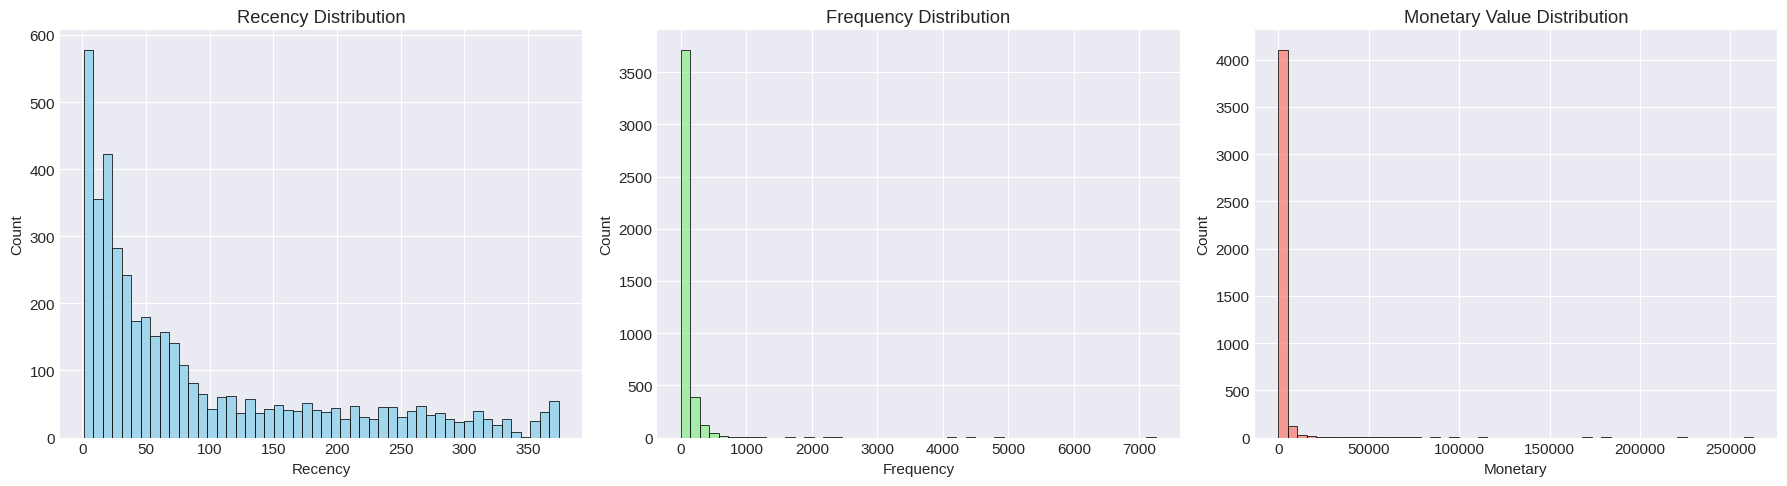
\includegraphics[width=\textwidth]{figures/fig_024_01.png}
  \caption{Marginal distributions of Recency (days since last purchase), Frequency
           (number of invoices), and Monetary value (GBP). All three variables show
           strong right-skewness, requiring log-transformation prior to clustering.}
  \label{fig:rfm_dist}
\end{figure}

\begin{table}[H]
  \centering
  \caption{Summary statistics of RFM features for the 4,306 retained customers.}
  \label{tab:rfm_stats}
  \begin{tabular}{lrrr}
    \toprule
    \textbf{Statistic} & \textbf{Recency (days)} & \textbf{Frequency} & \textbf{Monetary (\pounds)} \\
    \midrule
    Mean   & 92.36  & 83.27  & 1,775.39 \\
    Std    & 99.95  & 208.12 & 8,105.94 \\
    Min    & 1      & 1      & 3.75     \\
    Q1     & 18     & 15     & 251.48   \\
    Median & 51     & 37     & 566.38   \\
    Q3     & 141    & 91     & 1,436.84 \\
    Max    & 374    & 7,254  & 262,583  \\
    \bottomrule
  \end{tabular}
\end{table}

\subsection{Distribution of All Engineered Features}

Figure~\ref{fig:feat_dist} plots histograms for all eight features.  The skewness
statistics reveal extreme departures from normality: \texttt{Avg\_Quantity} (skewness
47.5), \texttt{Avg\_Order\_Value} (42.5), and \texttt{Monetary} (19.8) are the most
severely skewed, while \texttt{Customer\_Lifetime\_Days} (0.46) approaches symmetry.

\begin{figure}[H]
  \centering
  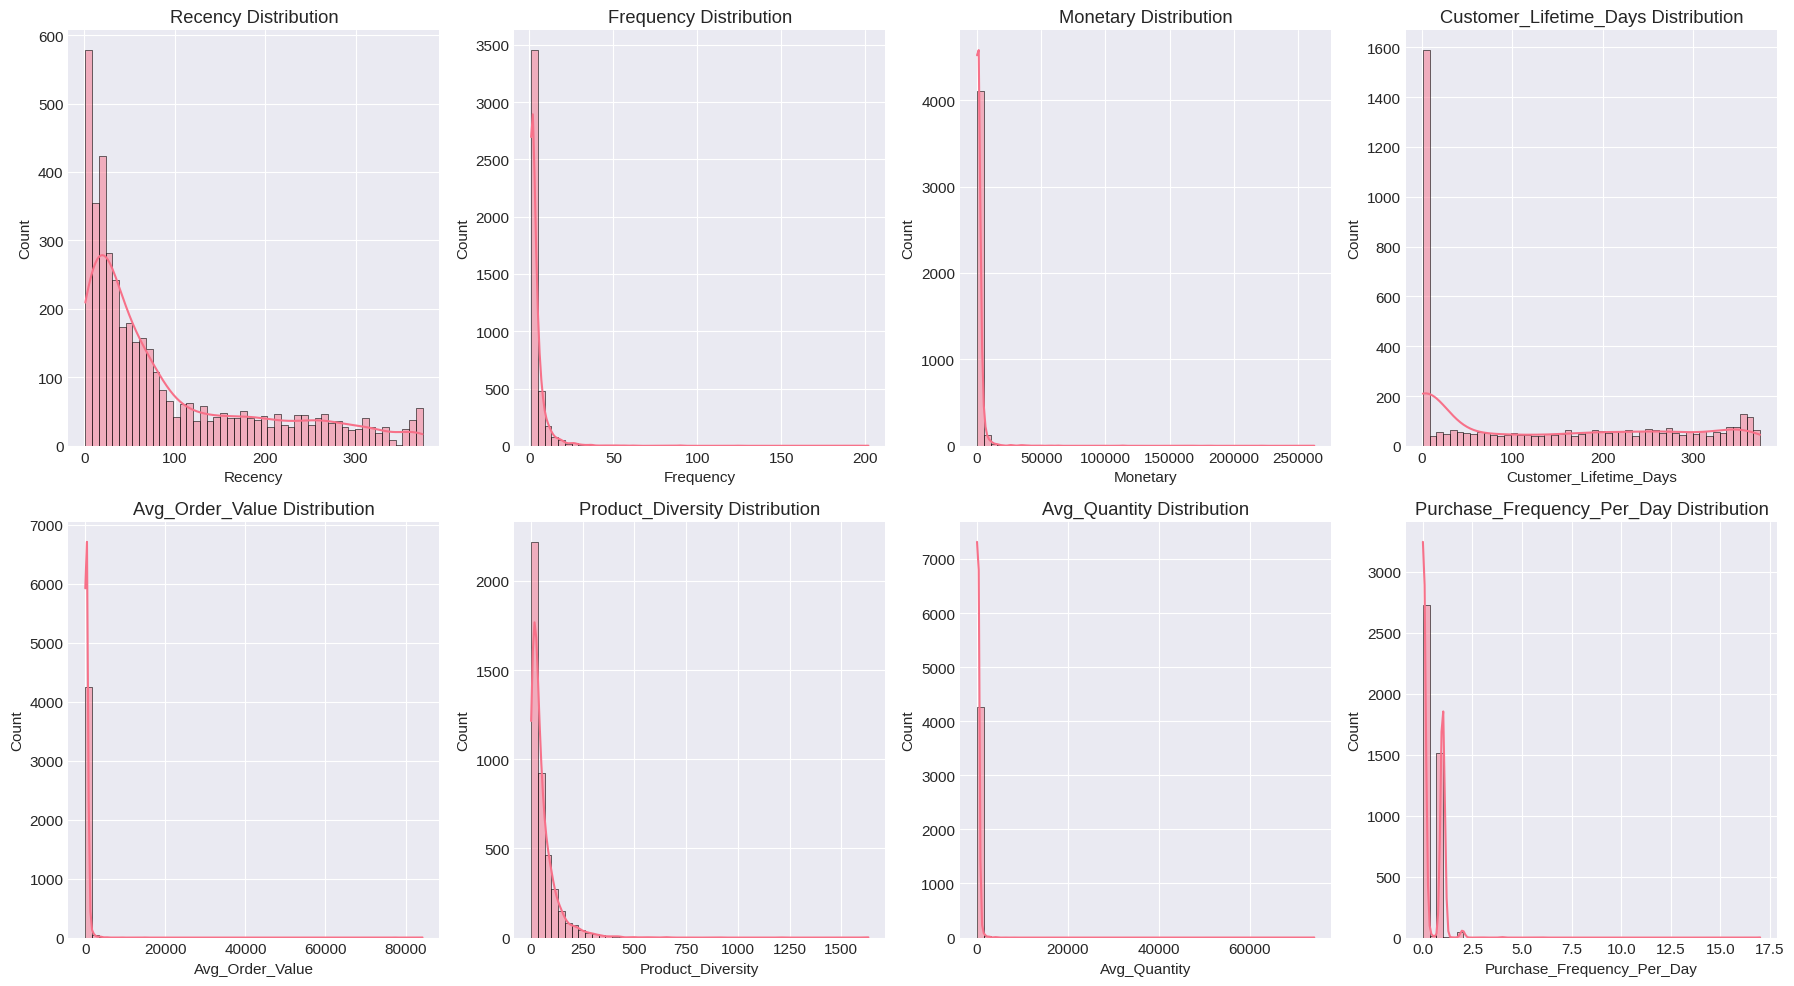
\includegraphics[width=\textwidth]{figures/fig_027_02.png}
  \caption{Distribution histograms for all eight engineered features.  Strong right-skewness
           in spending and transactional frequency metrics necessitates log-transformation
           to avoid scale dominance in distance-based clustering.}
  \label{fig:feat_dist}
\end{figure}

\subsection{Correlation Structure}

Figure~\ref{fig:corr} presents the pairwise Pearson correlation matrix.  The most
notable finding is the near-perfect positive correlation between
\texttt{Avg\_Order\_Value} and \texttt{Avg\_Quantity} ($r = 0.94$), indicating that
customers who order more items per transaction also spend more per order.
\texttt{Frequency} is moderately correlated with \texttt{Product\_Diversity} ($r = 0.69$)
and \texttt{Monetary} ($r = 0.53$), confirming that frequent buyers also tend to
explore more product categories and generate higher total revenue.
\texttt{Recency} shows negative correlation with \texttt{Frequency} ($r \approx -0.35$),
consistent with the expectation that recently active customers tend to purchase more
frequently.

\begin{figure}[H]
  \centering
  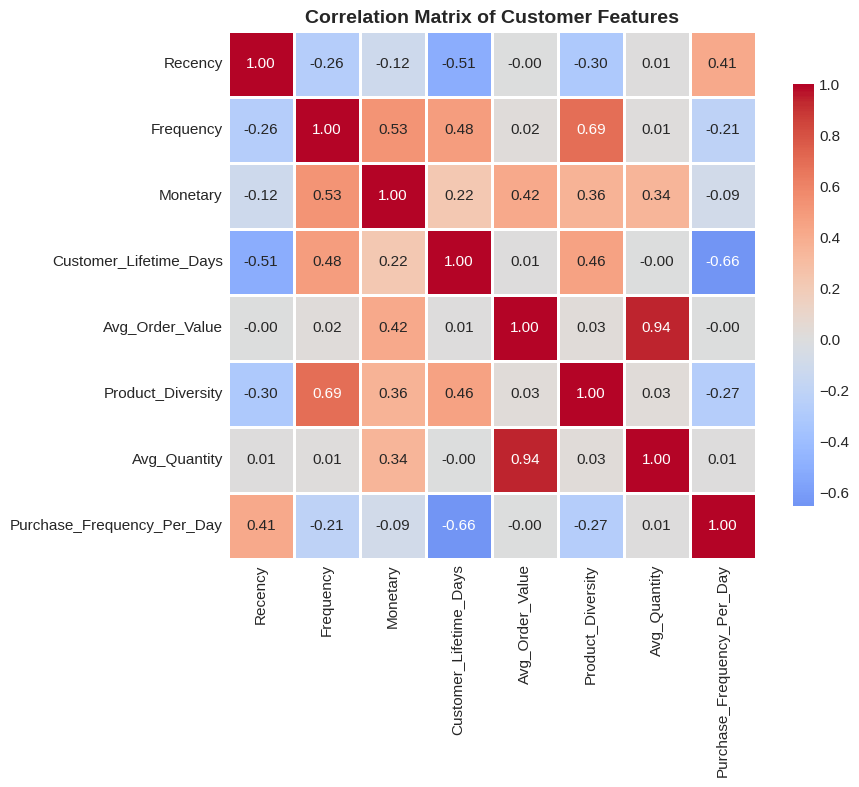
\includegraphics[width=0.78\textwidth]{figures/fig_029_03.png}
  \caption{Pearson correlation heatmap of the eight customer features.
           The strong \texttt{Avg\_Order\_Value}--\texttt{Avg\_Quantity} collinearity
           ($r=0.94$) motivates dimensionality reduction via PCA.}
  \label{fig:corr}
\end{figure}

\subsection{Outlier Analysis}

Boxplots (Figure~\ref{fig:boxplots}) and the IQR-based outlier summary confirm that
outliers are present in nearly all features, with \texttt{Monetary} having the
highest proportion (9.61\%) and \texttt{Frequency} 6.34\%.  Critically, these outliers
are not data quality issues---they represent genuinely high-value customers.
Accordingly, we retain them through clustering, as their discovery as a distinct
segment is a primary analytical objective.

\begin{figure}[H]
  \centering
  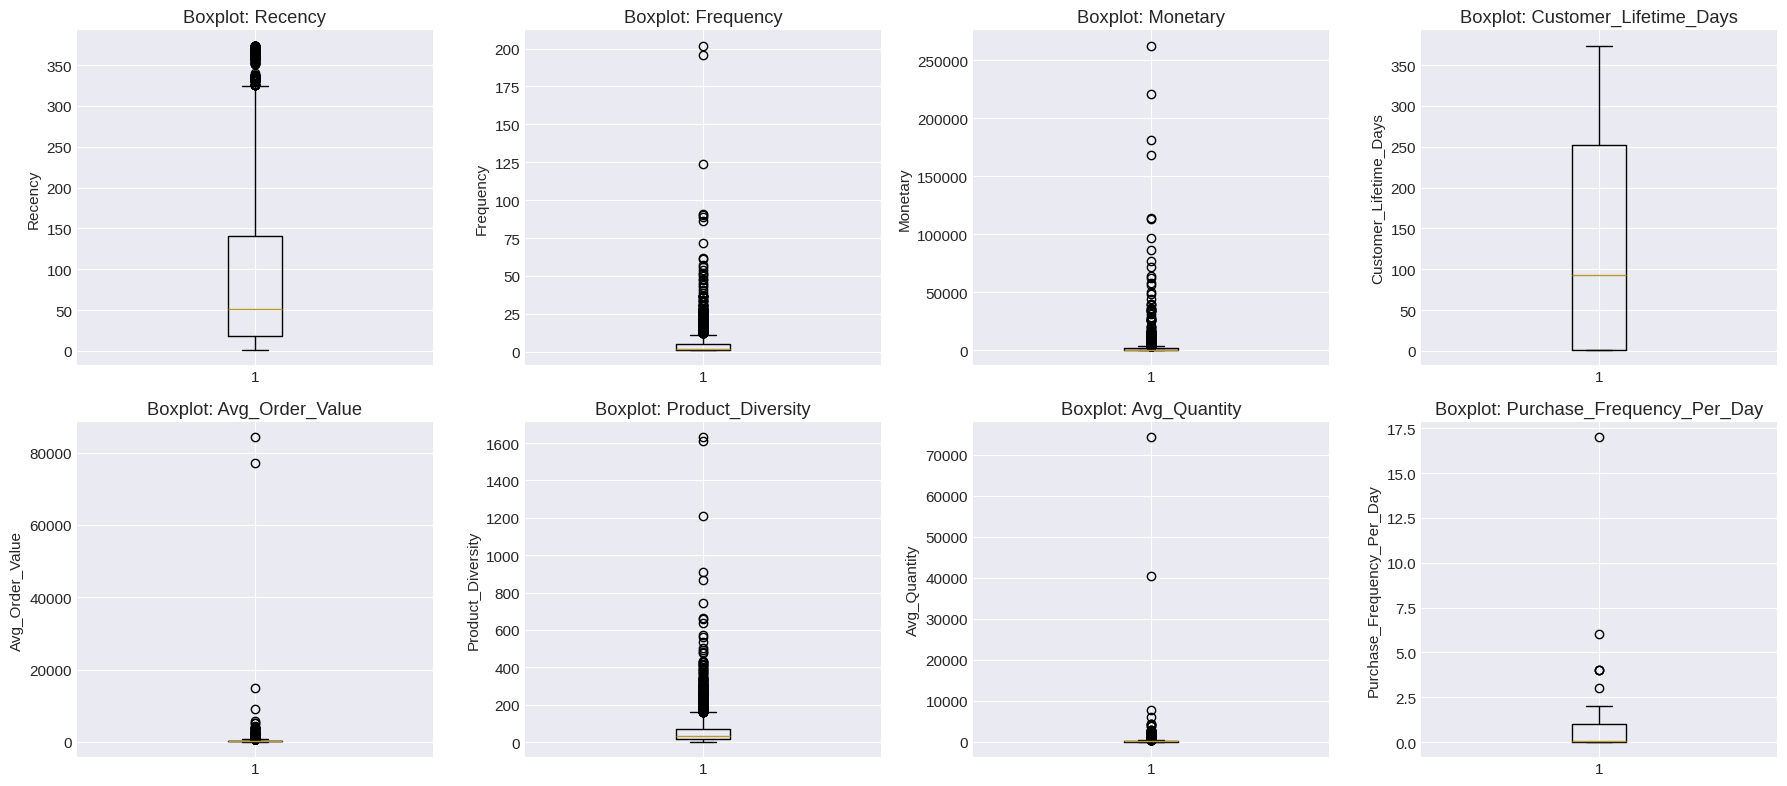
\includegraphics[width=\textwidth]{figures/fig_034_04.png}
  \caption{Boxplots illustrating outlier prevalence across all eight features.
           Outliers in \texttt{Monetary} and \texttt{Frequency} represent high-value
           customers and are intentionally retained for segmentation.}
  \label{fig:boxplots}
\end{figure}

\begin{table}[H]
  \centering
  \caption{Outlier counts and percentages (IQR method, $1.5\times$ fence).}
  \label{tab:outliers}
  \begin{tabular}{lrr}
    \toprule
    \textbf{Feature} & \textbf{Outlier Count} & \textbf{Percentage (\%)} \\
    \midrule
    Recency                     & 162 & 3.76 \\
    Frequency                   & 273 & 6.34 \\
    Monetary                    & 414 & 9.61 \\
    Customer\_Lifetime\_Days    &   0 & 0.00 \\
    Avg\_Order\_Value           & 287 & 6.67 \\
    Product\_Diversity          & 290 & 6.73 \\
    Avg\_Quantity               & 262 & 6.08 \\
    Purchase\_Frequency\_Per\_Day &   6 & 0.14 \\
    \bottomrule
  \end{tabular}
\end{table}

\subsection{Feature Relationship Patterns}

Figure~\ref{fig:scatter} presents scatter plots of key feature pairs.  The
Recency vs.\ Frequency plot reveals a non-linear inverse relationship: customers
who purchased recently tend to be frequent buyers, while the most inactive customers
(high recency) are almost exclusively low-frequency.  The Monetary vs.\ Frequency
plot shows a power-law-like concentration---most customers cluster in the low-frequency,
low-monetary corner, with a handful of extreme-value outliers representing the
commercially critical Champion segment.

\begin{figure}[H]
  \centering
  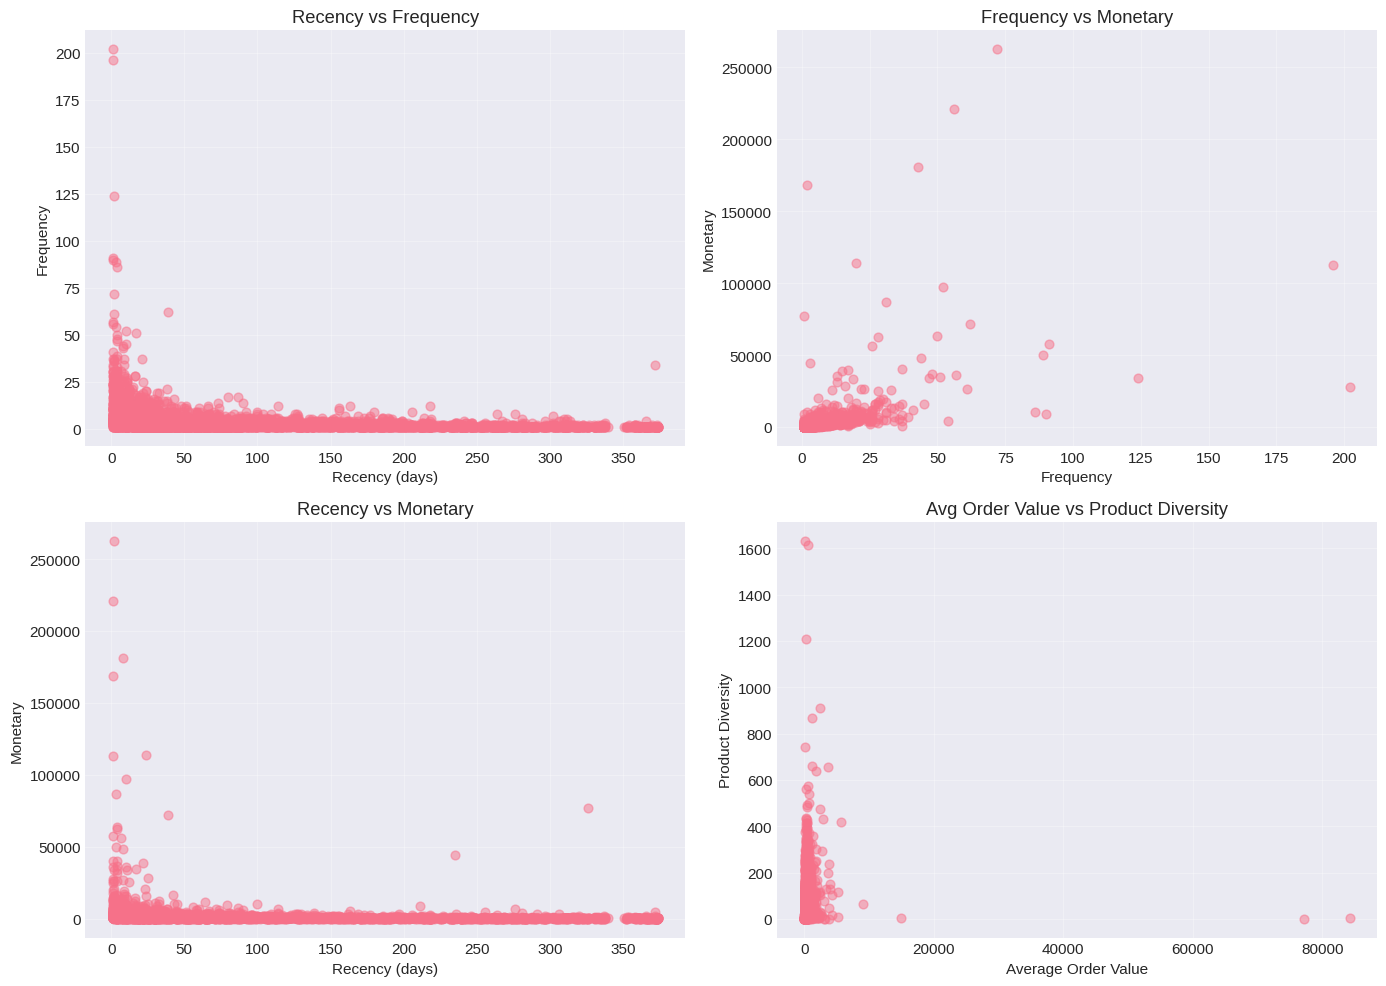
\includegraphics[width=\textwidth]{figures/fig_036_05.png}
  \caption{Pairwise scatter plots of key feature combinations.  The Recency--Frequency
           anti-correlation and the concentration of high-value customers in the
           extreme Monetary--Frequency region suggest the existence of at least
           two to three well-separated customer groups.}
  \label{fig:scatter}
\end{figure}

% ============================================================
\section{Statistical Analysis}
% ============================================================

\subsection{Data Transformation: Log-Scaling and Standardisation}

Distance-based clustering algorithms, including K-Means and hierarchical methods,
are sensitive to both the scale and the distributional shape of input features
\parencite{hastie2009elements}.  Features with larger numerical ranges dominate
the Euclidean distance metric, irrespective of their informational content.
Two preprocessing steps address this:

\textbf{Log Transformation:} We apply $x' = \ln(1 + x)$ (with $\varepsilon = 0.01$
added for numerical stability) to all features, reducing skewness from the range
$[0.46, 47.52]$ to approximately $[0, 0.5]$.  This transformation preserves the
ordering of customer values while compressing the influence of extreme observations.

\textbf{Standardisation:} Following log-transformation, we apply Z-score normalisation:
\[
  z = \frac{x' - \mu_{x'}}{\sigma_{x'}}
\]
so that each feature has mean $\approx 0$ and standard deviation $\approx 1$.
Figure~\ref{fig:transform} compares distributions before and after transformation.

\begin{figure}[H]
  \centering
  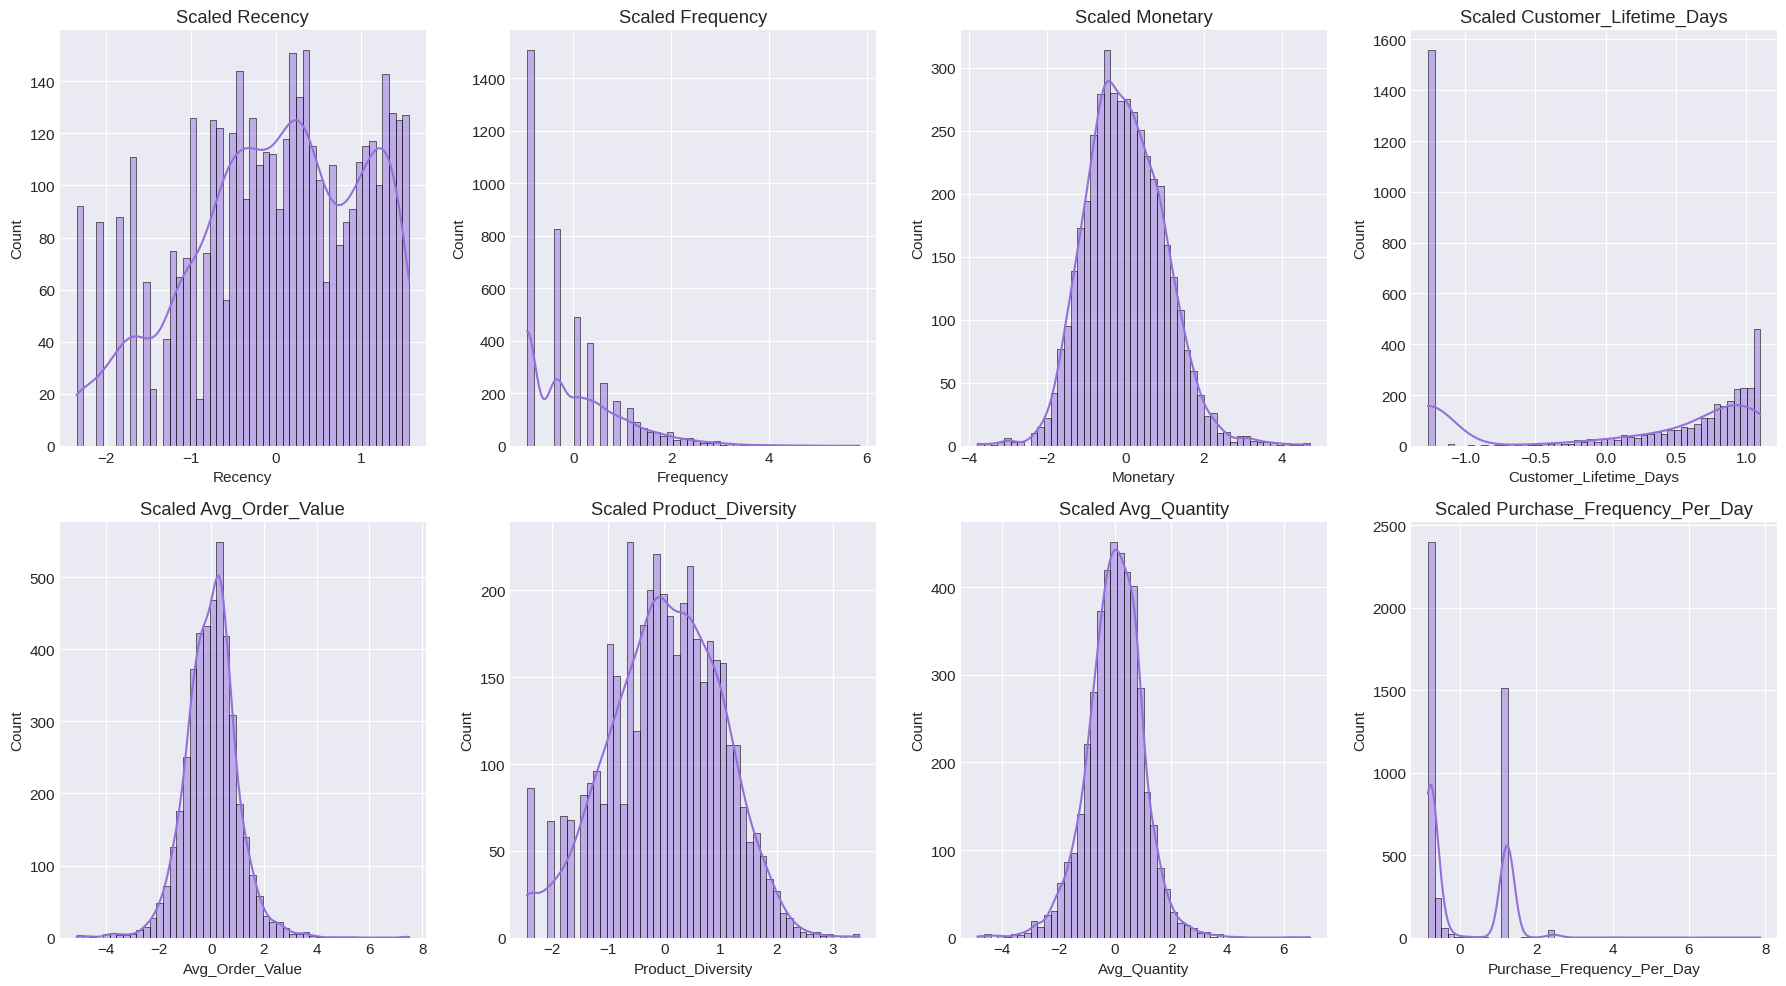
\includegraphics[width=\textwidth]{figures/fig_039_06.png}
  \caption{Feature distributions before (raw, left column) and after log-transformation
           and standardisation (right column).  Skewness is substantially reduced,
           making the data suitable for distance-based algorithms.}
  \label{fig:transform}
\end{figure}

\subsection{Principal Component Analysis}

With eight features exhibiting moderate-to-high correlations, direct clustering
risks double-counting correlated information.  PCA \parencite{jolliffe2016pca}
identifies orthogonal directions of maximum variance, reducing redundancy while
preserving discriminative structure.

\subsubsection{Variance Explained}

\begin{table}[H]
  \centering
  \caption{Variance explained by each principal component.}
  \label{tab:pca_var}
  \begin{tabular}{lrr}
    \toprule
    \textbf{Component} & \textbf{Variance (\%)} & \textbf{Cumulative (\%)} \\
    \midrule
    PC1 & 56.01 & 56.01 \\
    PC2 & 23.45 & 79.46 \\
    PC3 &  8.37 & 87.84 \\
    PC4 &  5.75 & 93.59 \\
    PC5 &  4.50 & 98.09 \\
    PC6 &  1.50 & 99.59 \\
    PC7 &  0.39 & 99.99 \\
    PC8 &  0.01 & 100.00\\
    \bottomrule
  \end{tabular}
\end{table}

Four components suffice to explain 93.59\% of total variance, enabling a reduction
from eight to four dimensions with minimal information loss (Figure~\ref{fig:pca_var}).

\begin{figure}[H]
  \centering
  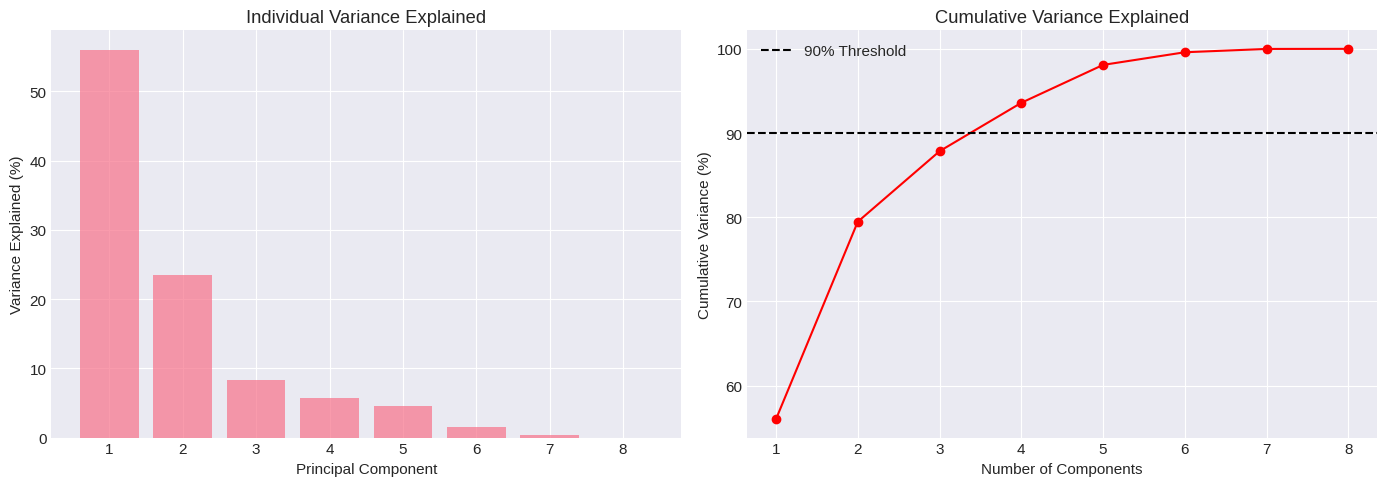
\includegraphics[width=\textwidth]{figures/fig_046_07.png}
  \caption{(Left) Scree plot of variance explained per principal component.
           (Right) Cumulative variance explained.  The four-component solution
           captures 93.59\% of total variance, representing the optimal
           complexity--interpretability trade-off.}
  \label{fig:pca_var}
\end{figure}

\subsubsection{Component Interpretation}

Table~\ref{tab:pca_loadings} and Figure~\ref{fig:pca_load} present the PCA loading
matrix.  \textbf{PC1} (56.01\% variance) loads positively on Frequency, Monetary,
Customer\_Lifetime\_Days, and Product\_Diversity, and negatively on Recency---it
represents overall customer value and engagement.  \textbf{PC2} (23.45\%) is dominated
by positive loadings on Avg\_Order\_Value and Avg\_Quantity---it captures basket size
behaviour, separating high-spend-per-visit customers from frequent-but-low-value ones.
\textbf{PC3} (8.37\%) reflects recency dynamics (positive loading on Recency, negative
on Purchase\_Frequency\_Per\_Day).  \textbf{PC4} (5.75\%) is largely driven by
Product\_Diversity, capturing product breadth independent of overall spending.

\begin{table}[H]
  \centering
  \caption{PCA loading matrix: feature contributions to the four retained components.}
  \label{tab:pca_loadings}
  \begin{tabular}{lrrrr}
    \toprule
    \textbf{Feature} & \textbf{PC1} & \textbf{PC2} & \textbf{PC3} & \textbf{PC4} \\
    \midrule
    Recency                     & $-$0.299 & 0.182 & 0.810 & 0.430 \\
    Frequency                   &    0.396 & $-$0.238 & $-$0.111 & 0.290 \\
    Monetary                    &    0.443 & 0.174 & 0.014 & 0.057 \\
    Customer\_Lifetime\_Days    &    0.394 & $-$0.323 & 0.329 & $-$0.177 \\
    Avg\_Order\_Value           &    0.261 & 0.581 & 0.080 & $-$0.178 \\
    Product\_Diversity          &    0.375 & 0.048 & $-$0.122 & 0.722 \\
    Avg\_Quantity               &    0.250 & 0.578 & 0.055 & $-$0.193 \\
    Purchase\_Freq\_Per\_Day    & $-$0.361 & 0.320 & $-$0.447 & 0.326 \\
    \bottomrule
  \end{tabular}
\end{table}

\begin{figure}[H]
  \centering
  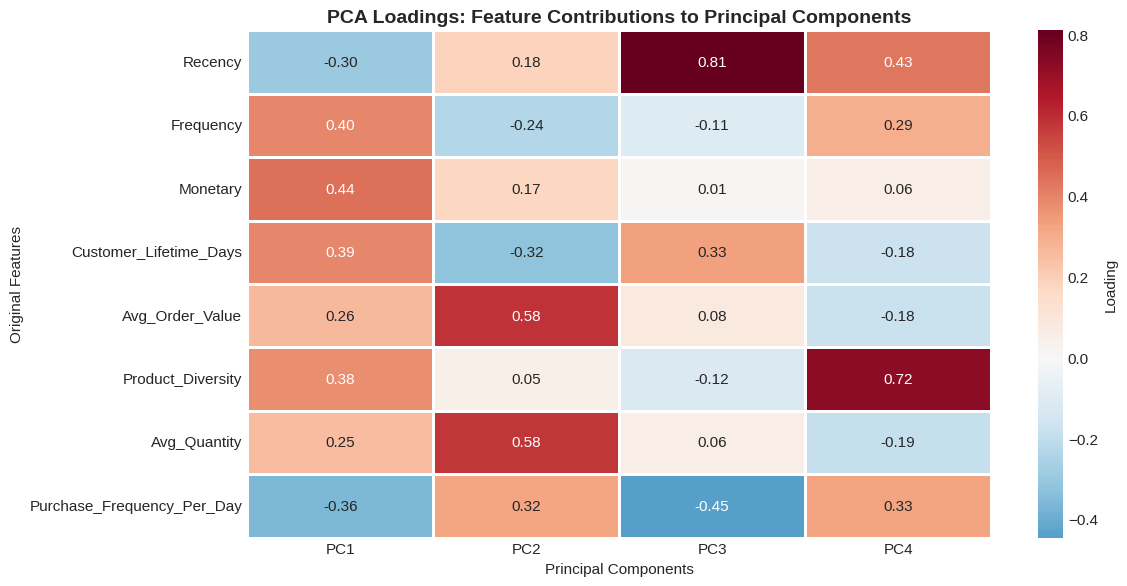
\includegraphics[width=\textwidth]{figures/fig_047_08.png}
  \caption{(Left) PCA biplot showing customer projections onto PC1 and PC2.
           (Right) Heatmap of loadings for the four retained components.
           PC1 cleanly separates high-value from low-value customers; PC2
           distinguishes basket-size behaviour.}
  \label{fig:pca_load}
\end{figure}

% ============================================================
\section{Models Used}
% ============================================================

\subsection{K-Means Clustering}

\subsubsection{Algorithm}

K-Means \parencite{macqueen1967} partitions $n$ observations into $k$ clusters by
iteratively minimising the within-cluster sum of squares (WCSS):
\[
  \underset{\{S_j\}}{\arg\min} \sum_{j=1}^{k} \sum_{\mathbf{x} \in S_j}
  \|\mathbf{x} - \boldsymbol{\mu}_j\|^2
\]
where $\boldsymbol{\mu}_j$ is the centroid of cluster $S_j$.  We use
\texttt{n\_init=20} random restarts and \texttt{max\_iter=300} to mitigate sensitivity
to initialisation, with \texttt{random\_state=42} for reproducibility.

\subsubsection{Optimal $k$ Selection}

Two complementary methods guide the choice of $k$ (Figure~\ref{fig:elbow}):

\begin{itemize}[leftmargin=*]
  \item \textbf{Elbow Method}: WCSS decreases steeply from $k=2$ to $k=4$, with the
        rate of decrease slowing markedly at $k=3$, suggesting the natural elbow.
  \item \textbf{Silhouette Analysis}: The average silhouette score peaks or shows a
        local maximum at $k=3$, balancing cluster cohesion and separation.
\end{itemize}

Both methods converge on $k=3$ as the optimal number of clusters.

\begin{figure}[H]
  \centering
  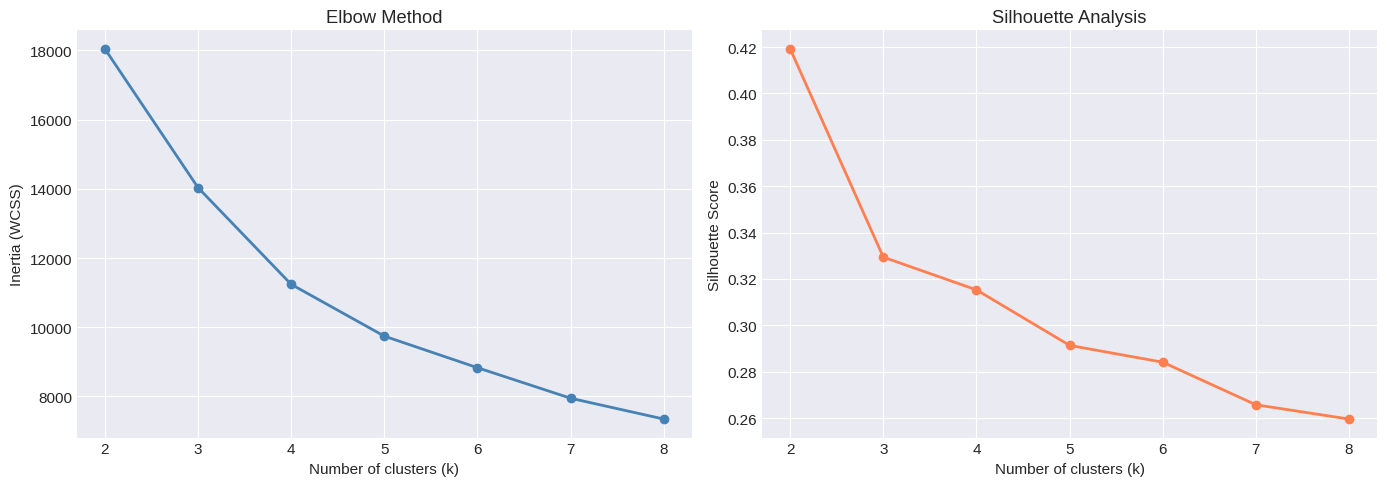
\includegraphics[width=\textwidth]{figures/fig_051_09.png}
  \caption{Cluster selection diagnostics.  (Left) Elbow plot: WCSS as a function of $k$.
           (Right) Silhouette scores for $k = 2, \ldots, 8$.  Both criteria support
           $k=3$ as the optimal cluster count.}
  \label{fig:elbow}
\end{figure}

\subsubsection{K-Means Results}

\begin{figure}[H]
  \centering
  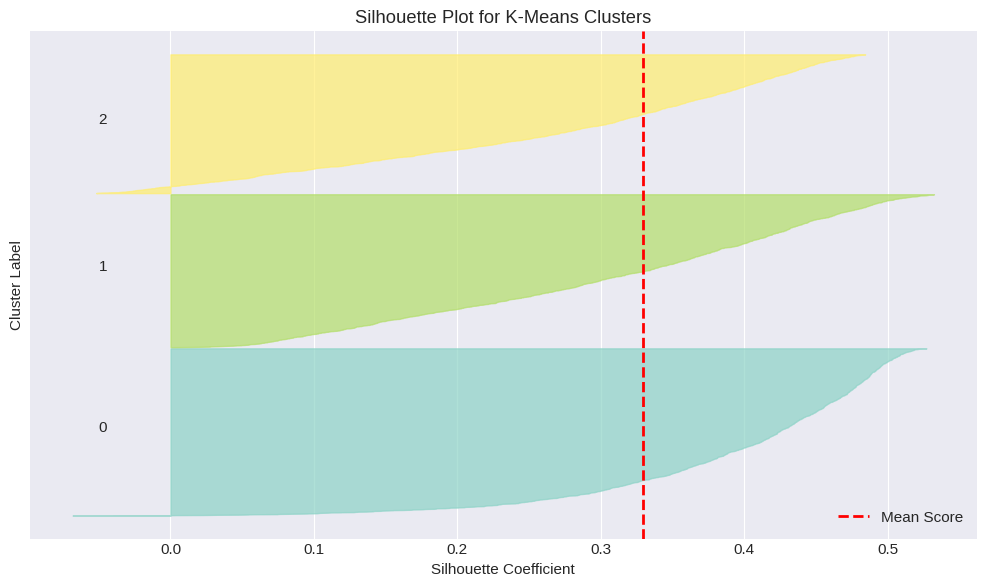
\includegraphics[width=0.75\textwidth]{figures/fig_054_10.png}
  \caption{K-Means cluster assignments projected onto the first two principal components.
           Three well-separated, roughly equal-sized groups are visible, with the
           Champion segment occupying the high PC1 region.}
  \label{fig:kmeans}
\end{figure}

K-Means with $k=3$ produces three clusters of comparable size:
\begin{itemize}[leftmargin=*]
  \item \textbf{Cluster 0}: 1,569 customers (36.4\%)
  \item \textbf{Cluster 1}: 1,435 customers (33.3\%)
  \item \textbf{Cluster 2}: 1,302 customers (30.2\%)
\end{itemize}
The Silhouette Score is \textbf{0.329} and the overall model achieves a
Calinski-Harabasz Index of \textbf{2,790.7}.

\subsection{Hierarchical Clustering}

\subsubsection{Algorithm}

Agglomerative hierarchical clustering \parencite{ward1963hierarchical} builds a
dendrogram by successively merging the two most similar clusters.  The linkage
criterion determines how inter-cluster distance is computed.  We evaluate four
linkage methods: \emph{Ward} (minimises within-cluster variance), \emph{Complete}
(maximum pairwise distance), \emph{Average} (mean pairwise distance), and
\emph{Single} (minimum pairwise distance).

Due to the computational expense of computing the full $4{,}306 \times 4{,}306$
linkage matrix, the dendrogram is generated on a representative subsample
(Figure~\ref{fig:dendro}).

\begin{figure}[H]
  \centering
  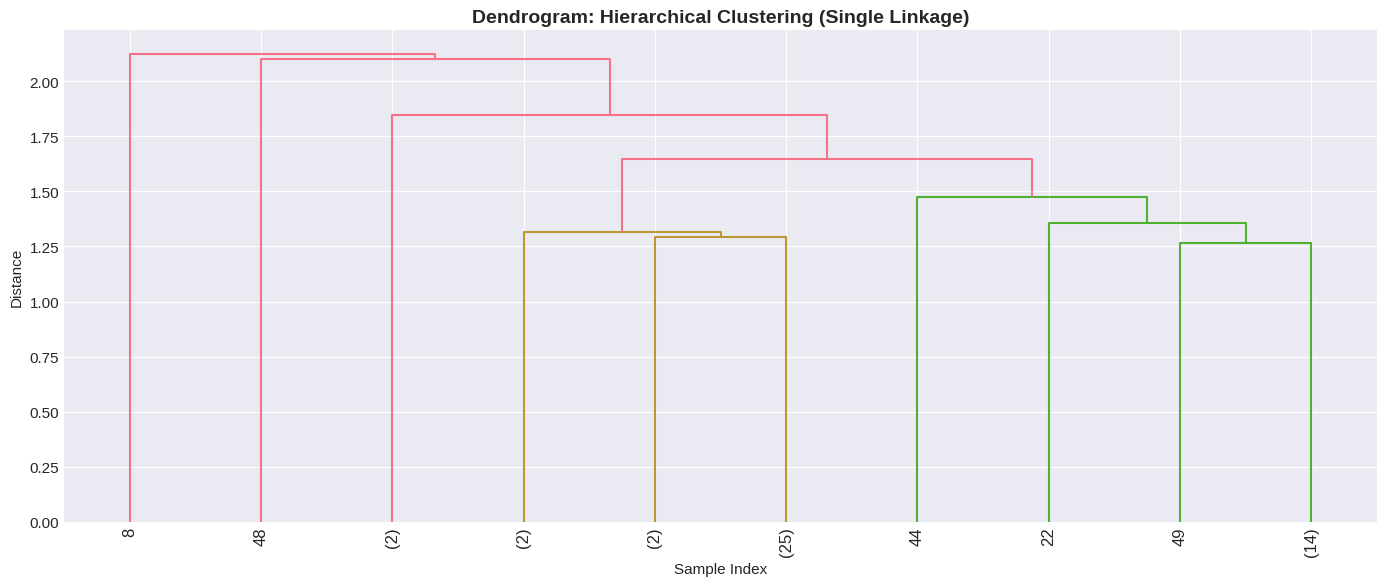
\includegraphics[width=\textwidth]{figures/fig_059_11.png}
  \caption{Truncated dendrogram from hierarchical clustering (Ward linkage, sample of
           4,306 observations).  The large vertical gap at height $\approx 10$--$12$
           supports three main clusters, consistent with the K-Means result.}
  \label{fig:dendro}
\end{figure}

\subsubsection{Linkage Method Comparison}

\begin{table}[H]
  \centering
  \caption{Silhouette scores across hierarchical linkage methods ($k=3$).}
  \label{tab:linkage}
  \begin{tabular}{lrl}
    \toprule
    \textbf{Linkage} & \textbf{Silhouette Score} & \textbf{Cluster Balance} \\
    \midrule
    Ward     & 0.324 & Balanced (practical) \\
    Complete & 0.252 & Moderate             \\
    Average  & 0.471 & Moderate             \\
    Single   & 0.677 & \emph{Degenerate} (4,304 / 1 / 1) \\
    \bottomrule
  \end{tabular}
\end{table}

Although single linkage achieves the highest nominal silhouette score (0.677),
it suffers from the well-known \emph{chaining effect}: essentially all customers
are assigned to one cluster, with two singleton outliers constituting the remaining
clusters.  This result is statistically valid but practically useless for business
segmentation.  Ward linkage produces the most balanced and actionable partition
(Silhouette = 0.324), closely matching the K-Means solution.

\subsection{DBSCAN Clustering}

\subsubsection{Algorithm}

DBSCAN \parencite{ester1996dbscan} is a density-based method that defines clusters
as high-density regions separated by low-density boundaries.  It requires two
hyperparameters: $\varepsilon$ (neighbourhood radius) and \texttt{min\_samples}
(minimum points to constitute a dense region).  Unlike K-Means, DBSCAN does not
require pre-specifying the number of clusters and can identify noise points
(customers who do not belong to any dense group).

\subsubsection{Parameter Tuning}

The $k$-distance graph (Figure~\ref{fig:kdist}) is used to identify the ``elbow''
that suggests an appropriate $\varepsilon$.  A grid search over
$\varepsilon \in \{0.3, 0.4, \ldots, 0.9\}$ and
$\texttt{min\_samples} \in \{3, 4, 5\}$ selects the combination maximising the
silhouette score: $\varepsilon = 0.7$, \texttt{min\_samples} = 5.

\begin{figure}[H]
  \centering
  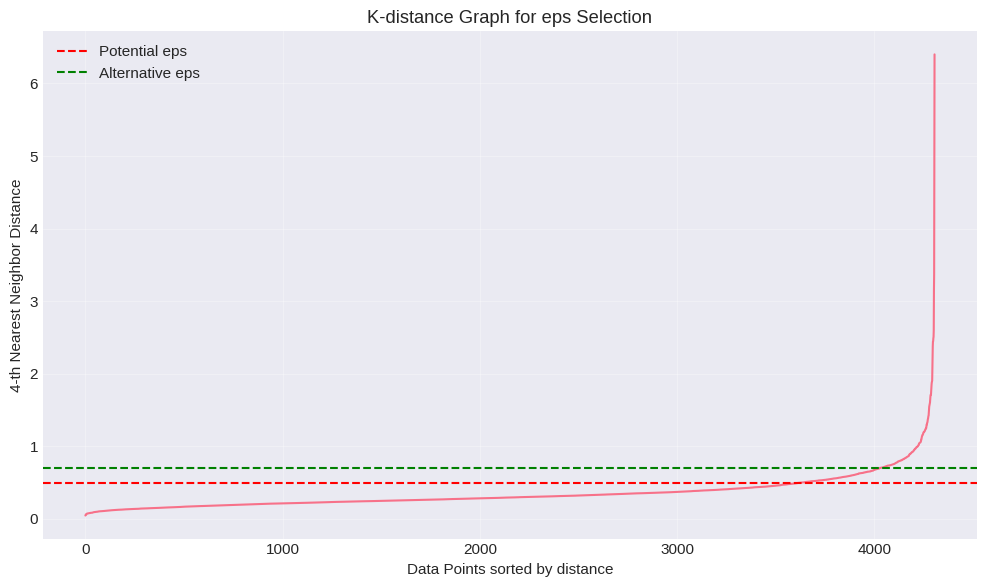
\includegraphics[width=0.7\textwidth]{figures/fig_064_12.png}
  \caption{$k$-distance graph used to identify the optimal DBSCAN $\varepsilon$ parameter.
           The elbow at approximately $\varepsilon = 0.7$ guides neighbourhood radius selection.}
  \label{fig:kdist}
\end{figure}

\subsubsection{DBSCAN Results}

With the tuned parameters, DBSCAN identifies three clusters and 100 noise points
(Figure~\ref{fig:dbscan}):

\begin{itemize}[leftmargin=*]
  \item \textbf{Noise points}: 100 (2.3\%)
  \item \textbf{Cluster 0}: 2,677 customers (62.2\%)
  \item \textbf{Cluster 1}: 1,525 customers (35.4\%)
  \item \textbf{Cluster 2}: 4 customers (0.1\%) --- micro-cluster of extreme outliers
\end{itemize}

\begin{figure}[H]
  \centering
  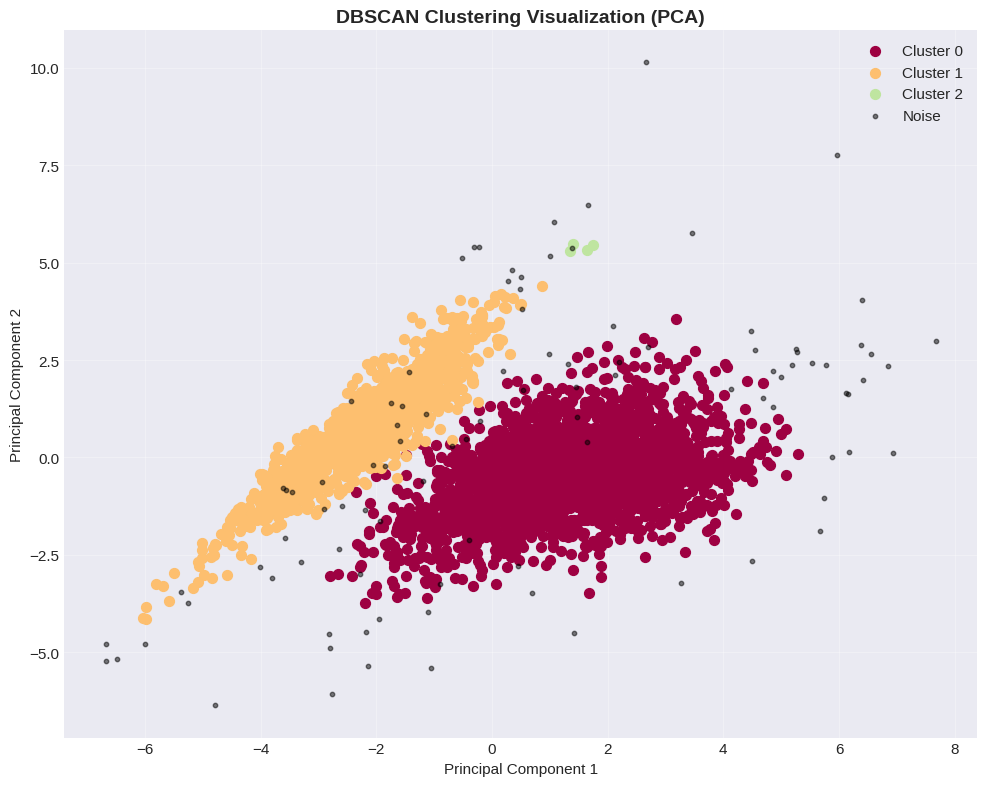
\includegraphics[width=0.7\textwidth]{figures/fig_067_13.png}
  \caption{DBSCAN cluster assignments projected onto PC1--PC2.  Noise points (grey)
           are concentrated at the boundary between the two main clusters.
           The micro-cluster (Cluster 2) captures extreme-value customers.}
  \label{fig:dbscan}
\end{figure}

DBSCAN achieves a Silhouette Score of 0.449 on the non-noise subset, but the heavily
imbalanced cluster sizes (62.2\% vs.\ 35.4\% vs.\ 0.1\%) reduce its practical utility
for balanced marketing segmentation.

\subsection{Supervised Validation: Logistic Regression}

\subsubsection{Rationale}

A supervised model trained to predict K-Means cluster labels from the original feature
space serves as a complementary validation: high accuracy confirms that cluster
boundaries align with geometrically coherent regions in the original feature space,
not just the PCA-compressed space used for clustering
\parencite{hastie2009elements}.

\subsubsection{Model Specification}

Two Logistic Regression variants are compared:
\begin{itemize}[leftmargin=*]
  \item \textbf{L2 (Ridge)}: Penalises $\|\boldsymbol{\beta}\|_2^2$; all features
        retain non-zero coefficients; promotes coefficient shrinkage.
  \item \textbf{L1 (Lasso)} \parencite{tibshirani1996lasso}: Penalises
        $\|\boldsymbol{\beta}\|_1$; produces sparse solutions by zeroing out
        irrelevant features; supports feature selection.
\end{itemize}

The dataset is split 80\%/20\% (train/test) with stratification, yielding
3,444 training and 862 test observations.  Five-fold cross-validation provides
variance estimates.

% ============================================================
\section{Results, Model Evaluation, and Key Insights}
% ============================================================

\subsection{Clustering Evaluation Metrics}

Three established metrics assess clustering quality \parencite{rousseeuw1987silhouettes,
davies1979cluster, calinski1974dendrite}:

\begin{itemize}[leftmargin=*]
  \item \textbf{Silhouette Score} ($\in [-1, 1]$): Higher is better; measures how
        similar each point is to its own cluster relative to the nearest other cluster.
  \item \textbf{Davies-Bouldin Index} ($\geq 0$): Lower is better; measures the ratio
        of within-cluster scatter to inter-cluster separation.
  \item \textbf{Calinski-Harabasz Index} ($\geq 0$): Higher is better; ratio of
        between-cluster to within-cluster dispersion.
\end{itemize}

\begin{table}[H]
  \centering
  \caption{Clustering algorithm comparison across three evaluation metrics.}
  \label{tab:cluster_compare}
  \begin{tabular}{lrrrrr}
    \toprule
    \textbf{Method} & \textbf{Silhouette}$\uparrow$ & \textbf{Davies-Bouldin}$\downarrow$
                    & \textbf{Calinski-Harabasz}$\uparrow$ & \textbf{Clusters} & \textbf{Noise} \\
    \midrule
    K-Means       & 0.329 & 1.148 & 2,790.7 & 3 & 0   \\
    Hierarchical  & 0.677 & 0.229 &    16.5 & 3 & 0   \\
    DBSCAN        & 0.449 & 0.740 & 1,818.4 & 3 & 100 \\
    \bottomrule
  \end{tabular}
\end{table}

\begin{figure}[H]
  \centering
  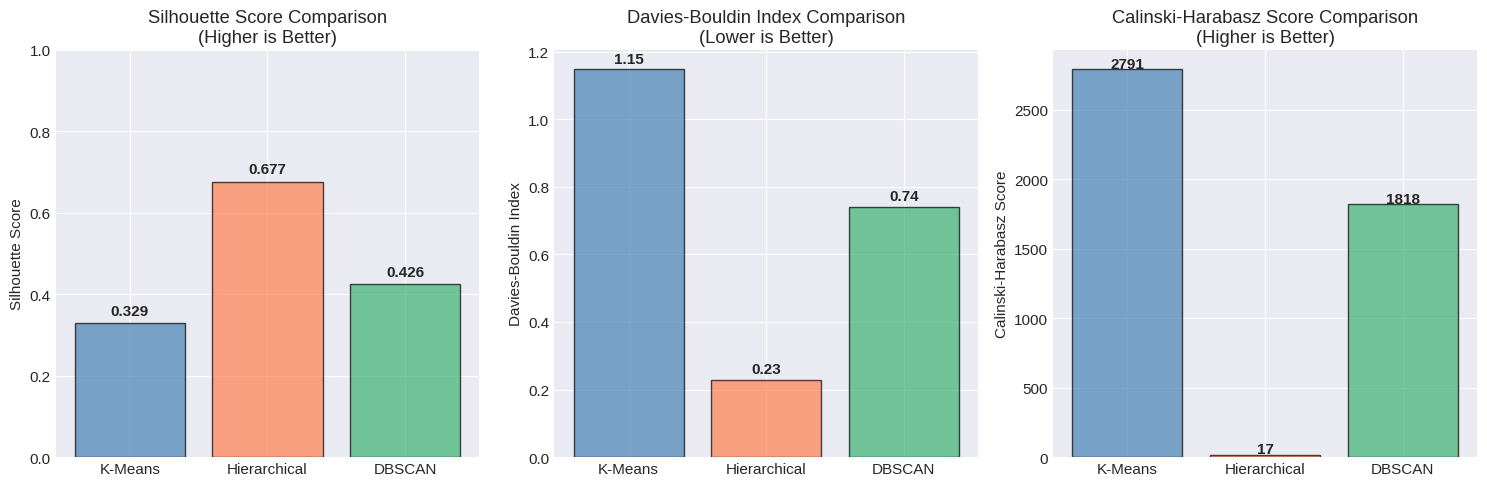
\includegraphics[width=\textwidth]{figures/fig_071_14.png}
  \caption{Side-by-side comparison of Silhouette Score, Davies-Bouldin Index, and
           Calinski-Harabasz Index across the three clustering methods.
           K-Means achieves the highest Calinski-Harabasz score, reflecting
           the best ratio of between-cluster to within-cluster dispersion.}
  \label{fig:compare}
\end{figure}

\textbf{Model Selection Rationale:} Hierarchical clustering's superior silhouette and
Davies-Bouldin scores are inflated by the single-linkage chaining artefact, where
near-perfect metric values reflect a degenerate (one massive cluster) solution rather
than genuine segmentation.  When Ward linkage is applied, hierarchical clustering
(Silhouette = 0.324, CH = 16.5) substantially underperforms K-Means
(CH = 2,790.7) on the Calinski-Harabasz criterion.  DBSCAN produces imbalanced
segments with a micro-cluster of four customers.  \textbf{K-Means with $k=3$ is
selected} as the final model on the grounds of balanced cluster sizes, highest
Calinski-Harabasz index, interpretable PCA-space separation, and practical
business utility.

\subsection{Cluster Profiles and Segment Interpretation}

\begin{table}[H]
  \centering
  \caption{Mean values of key features by K-Means cluster.}
  \label{tab:cluster_profiles}
  \begin{tabular}{lrrrrr}
    \toprule
    \textbf{Cluster} & \textbf{Recency} & \textbf{Frequency} & \textbf{Monetary (\pounds)}
                     & \textbf{Lifetime (days)} & \textbf{Customers} \\
    \midrule
    0 -- Hibernating  & 155.4 & 21.0  &    309 & 1.1    & 1,569 (36.4\%) \\
    1 -- Active/Loyal &  79.2 & 44.7  &    621 & 165.3  & 1,435 (33.3\%) \\
    2 -- Champions    &  30.9 & 200.9 &  4,815 & 250.5  & 1,302 (30.2\%) \\
    \bottomrule
  \end{tabular}
\end{table}

\subsubsection{Segment Characterisations}

\textbf{Cluster 0 -- Hibernating (36.4\%):} These customers have not purchased for
an average of 155 days, make relatively infrequent purchases (21 transactions), and
generate modest revenue (\pounds309 median).  Their near-zero Customer\_Lifetime\_Days
mean (1.1 days) suggests many are one-time or early-churn customers.  This segment
contributes only 6.4\% of total revenue.

\textbf{Cluster 1 -- Active/Loyal (33.3\%):} Moderate recency (79 days), moderate
frequency (45 transactions), and moderate monetary value (\pounds621).  A Customer
Lifetime of 165 days indicates established purchasing relationships.  These customers
represent a growth opportunity: with appropriate incentives, a subset may be
cultivated into Champions.  This segment generates 11.6\% of total revenue.

\textbf{Cluster 2 -- Champions (30.2\%):} The defining commercial asset of the
retailer.  Recency of only 31 days confirms active engagement; average frequency
of 201 transactions per customer is extraordinary; mean monetary value of \pounds4,815
reflects substantial lifetime spending.  Lifetime of 250 days shows these are
long-tenured, loyal customers.  This segment generates \textbf{82.0\%} of total
revenue despite comprising less than a third of the customer base.

\begin{table}[H]
  \centering
  \caption{Revenue contribution by K-Means cluster.}
  \label{tab:revenue}
  \begin{tabular}{lrrr}
    \toprule
    \textbf{Cluster} & \textbf{Total Revenue (\pounds)} & \textbf{Share (\%)} \\
    \midrule
    0 -- Hibernating  & 485,482   &  6.4 \\
    1 -- Active/Loyal & 890,573   & 11.6 \\
    2 -- Champions    & 6,268,769 & 82.0 \\
    \midrule
    \textbf{Total}    & \textbf{7,644,824} & \textbf{100.0} \\
    \bottomrule
  \end{tabular}
\end{table}

This 30--82 relationship is a manifestation of the Pareto principle and has direct
implications for resource allocation in retention and marketing campaigns.

\subsection{Supervised Validation Results}

\begin{table}[H]
  \centering
  \caption{Logistic Regression performance metrics on the held-out test set ($n=862$).}
  \label{tab:lr_results}
  \begin{tabular}{lcccc}
    \toprule
    \textbf{Model} & \textbf{Accuracy} & \textbf{Precision} & \textbf{Recall} & \textbf{F1} \\
    \midrule
    L2 (Ridge) & 0.9965 & 0.9966 & 0.9965 & 0.9965 \\
    L1 (Lasso) & 0.9872 & 0.9872 & 0.9872 & 0.9872 \\
    \bottomrule
  \end{tabular}
\end{table}

\begin{table}[H]
  \centering
  \caption{Five-fold cross-validation results (mean $\pm$ standard deviation).}
  \label{tab:cv_results}
  \begin{tabular}{lcccc}
    \toprule
    \textbf{Model} & \textbf{Accuracy} & \textbf{Precision} & \textbf{Recall} & \textbf{F1} \\
    \midrule
    L2 (Ridge) & $0.9945 \pm 0.0034$ & $0.9945 \pm 0.0033$ & $0.9945 \pm 0.0034$ & $0.9945 \pm 0.0034$ \\
    L1 (Lasso) & $0.9927 \pm 0.0028$ & $0.9928 \pm 0.0027$ & $0.9927 \pm 0.0028$ & $0.9927 \pm 0.0027$ \\
    \bottomrule
  \end{tabular}
\end{table}

\begin{figure}[H]
  \centering
  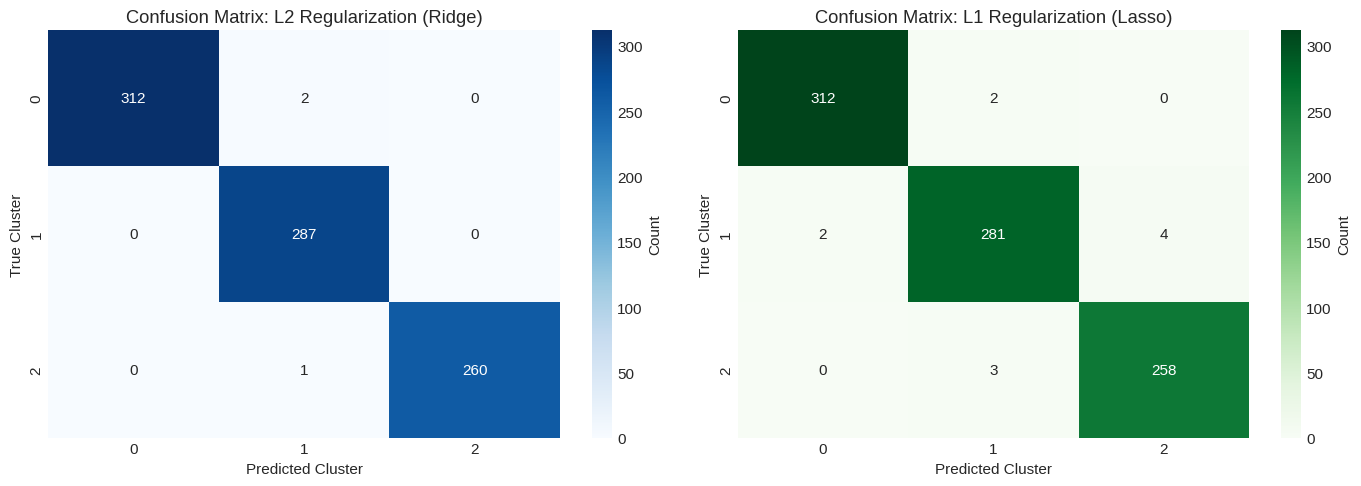
\includegraphics[width=\textwidth]{figures/fig_084_15.png}
  \caption{Confusion matrices for (left) L2 and (right) L1 Logistic Regression on the
           test set.  Both models achieve near-perfect classification, with
           misclassifications predominantly at the Cluster 0/1 boundary, consistent
           with the moderate Silhouette Score.}
  \label{fig:cm}
\end{figure}

The near-perfect accuracy (L2: 99.65\%, L1: 98.72\%) confirms that the K-Means
clusters correspond to geometrically coherent regions in the original eight-dimensional
feature space---not artefacts of the PCA compression.

\begin{figure}[H]
  \centering
  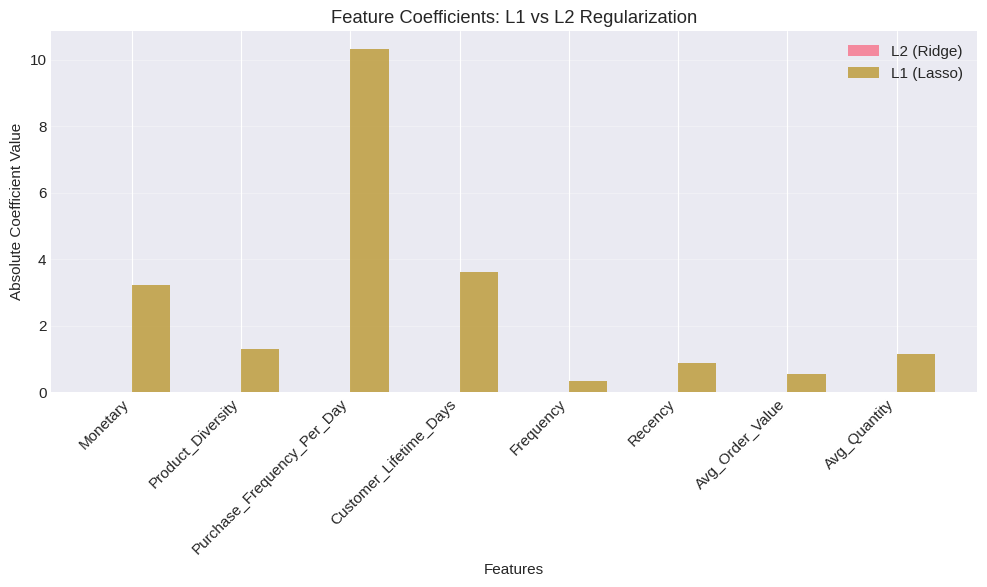
\includegraphics[width=0.75\textwidth]{figures/fig_085_16.png}
  \caption{Absolute feature coefficients from L1 Logistic Regression, revealing the
           most discriminative features.  \texttt{Purchase\_Frequency\_Per\_Day} (10.33),
           \texttt{Monetary} (3.22), and \texttt{Customer\_Lifetime\_Days} (3.62)
           are the strongest predictors of cluster membership.}
  \label{fig:feature_imp}
\end{figure}

The L1 model's sparse solution (Figure~\ref{fig:feature_imp}) identifies
\texttt{Purchase\_Frequency\_Per\_Day}, \texttt{Customer\_Lifetime\_Days}, and
\texttt{Monetary} as the most discriminative features, aligning intuitively with
the cluster definitions: Champions are distinguished precisely by their purchase
rate, tenure, and spending.

% ============================================================
\section{Challenges, Limitations, and Societal Impact}
% ============================================================

\subsection{Methodological Challenges}

\textbf{Extreme feature skewness.} Raw RFM and behavioural features exhibit skewness
values up to 47.5, far beyond the typical range amenable to distance-based algorithms.
Log-transformation substantially mitigated this, but residual distributional asymmetry
may still bias cluster shapes.

\textbf{K-Means sensitivity to initialisation.} Despite 20 random restarts, K-Means
convergence to a global optimum is not guaranteed.  The consistency of results across
multiple seeds suggests stability, but alternative methods (e.g., K-Means++ initialisation)
could further reduce this risk.

\textbf{PCA information loss.} Retaining four components preserves 93.59\% of variance,
but the remaining 6.41\% may contain meaningful signals for fine-grained segmentation.
Customers near cluster boundaries in PCA space may be misassigned relative to their
true position in the original feature space---an issue partially addressed by the
high supervised validation accuracy.

\textbf{DBSCAN scalability.} DBSCAN's quadratic distance computation was computationally
intensive for $n=4,306$ customers in four-dimensional PCA space.  For larger datasets,
approximate nearest-neighbour methods would be required.

\textbf{Single-linkage degenerate solution.} The chaining effect in single-linkage
hierarchical clustering produced a nominally high silhouette score from a practically
useless partition.  This underscores the importance of evaluating clustering solutions
for business utility, not just statistical metrics.

\subsection{Dataset Limitations}

\begin{itemize}[leftmargin=*]
  \item \textbf{Temporal scope}: One year of data cannot distinguish seasonality from
        genuine churn.  The Hibernating segment may include seasonal buyers who would
        return in December 2012.
  \item \textbf{Geographically skewed}: The UK comprises the vast majority of customers;
        international segmentation may not be generalisable.
  \item \textbf{Missing CustomerIDs}: The 24.93\% of transactions without a CustomerID
        (likely guest checkouts) are excluded entirely.  If their behaviour systematically
        differs from registered customers, the analysis understates the full customer base.
  \item \textbf{B2B/B2C mix}: The retailer sells to both individual consumers and resellers.
        The Champion segment likely contains a disproportionate share of B2B resellers,
        whose high frequency and monetary values reflect wholesale rather than consumer behaviour.
\end{itemize}

\subsection{Societal and Ethical Considerations}

Automated customer segmentation raises several ethical considerations.  Segment-based
differential treatment (e.g., different pricing, service levels, or communication
frequency) can inadvertently encode demographic proxies if purchasing behaviour
correlates with protected characteristics such as income, geography, or age.
In the absence of demographic data, direct proxy discrimination cannot be assessed,
but this risk should be monitored when deploying recommendations in practice.

Furthermore, retention strategies targeting the Hibernating segment must be designed
transparently: unsolicited reactivation campaigns may violate GDPR opt-out provisions
if customers have not consented to marketing communications.

% ============================================================
\section{Conclusion, Future Work, and Reproducibility}
% ============================================================

\subsection{Conclusion}

This analysis has transformed 541,909 raw transactional records into a statistically
rigorous, business-actionable three-segment customer model.  The key findings are:

\begin{enumerate}[leftmargin=*]
  \item \textbf{Three distinct customer segments} emerge robustly from the data:
        Hibernating (36.4\%), Active/Loyal (33.3\%), and Champions (30.2\%).
  \item \textbf{Champions generate 82\% of revenue} despite comprising less than a
        third of the customer base, confirming a strong Pareto effect.
  \item \textbf{K-Means outperforms} Hierarchical and DBSCAN clustering for practical
        segmentation on this dataset, producing balanced, coherent, and interpretable groups.
  \item \textbf{PCA dimensionality reduction} to four components (93.59\% variance)
        enables efficient clustering without material information loss.
  \item \textbf{Logistic regression validation} (L2: 99.65\% accuracy) confirms that
        segments are geometrically coherent in the original feature space.
\end{enumerate}

\subsection{Business Recommendations}

\textbf{Champions (Cluster 2)}:
\begin{itemize}[leftmargin=*,noitemsep]
  \item Enrol in exclusive VIP loyalty programmes with early product access and
        dedicated account management.
  \item Provide personalised product recommendations based on their broad product
        diversity (mean 37+ categories).
  \item Monitor for any increase in Recency as an early warning of churn.
\end{itemize}

\textbf{Active/Loyal (Cluster 1)}:
\begin{itemize}[leftmargin=*,noitemsep]
  \item Deploy tiered incentive programmes (e.g., spend \pounds X more this quarter
        to unlock Champion status) to nudge conversion upward.
  \item Introduce cross-category promotions to increase Product\_Diversity, a key
        differentiator of Champions.
  \item Run targeted upsell campaigns leveraging their established purchase history.
\end{itemize}

\textbf{Hibernating (Cluster 0)}:
\begin{itemize}[leftmargin=*,noitemsep]
  \item Deploy GDPR-compliant win-back email campaigns with time-limited discounts
        for customers with Recency $>$ 90 days.
  \item Segment further by Customer\_Lifetime\_Days to distinguish newly acquired but
        never-repurchased customers from formerly active lapsed buyers.
  \item Set an automated churn threshold: customers exceeding 200 days without a
        purchase may be cost-effectively deprioritised.
\end{itemize}

\subsection{Future Work}

\begin{itemize}[leftmargin=*]
  \item \textbf{Temporal segmentation}: Extend to multi-period RFM to capture
        segment migration over time (e.g., customers transitioning from Active to
        Hibernating).
  \item \textbf{Product-level features}: Incorporate category-level purchasing patterns
        to identify product affinity clusters within the existing RFM segments.
  \item \textbf{Gaussian Mixture Models}: Explore soft clustering to probabilistically
        assign boundary customers to multiple segments, enabling gradient marketing strategies.
  \item \textbf{International sub-segmentation}: Separate UK and international
        customers before clustering, given potential B2B/B2C confounds.
  \item \textbf{Real-time scoring pipeline}: Deploy the trained Logistic Regression
        model as a production API to score new customers as they cross feature thresholds.
\end{itemize}

\subsection{Reproducibility}

\textbf{Environment:}
\begin{verbatim}
Python        3.x
pandas        >= 1.3
numpy         >= 1.21
scikit-learn  >= 1.0
matplotlib    >= 3.4
seaborn       >= 0.11
scipy         >= 1.7
\end{verbatim}

\textbf{To reproduce the analysis:}
\begin{enumerate}[leftmargin=*]
  \item Clone or download the project directory.
  \item Install dependencies: \texttt{pip install pandas numpy scikit-learn
        matplotlib seaborn scipy openpyxl}.
  \item Open \texttt{Main\_STAT654\_Customer\_Segmentation\_Final.ipynb} in
        Jupyter Notebook or JupyterLab.
  \item Run all cells sequentially (\textit{Kernel} $\to$ \textit{Restart and Run All}).
\end{enumerate}

\textbf{File structure:}
\begin{verbatim}
.
├── Main_STAT654_Customer_Segmentation_Final.ipynb
└── report/
    ├── main.tex
    ├── references.bib
    └── figures/
        ├── fig_024_01.png   # RFM distributions
        ├── fig_027_02.png   # All-feature distributions
        ├── fig_029_03.png   # Correlation heatmap
        ├── fig_034_04.png   # Outlier boxplots
        ├── fig_036_05.png   # Feature scatter plots
        ├── fig_039_06.png   # Log-transform comparison
        ├── fig_046_07.png   # PCA scree / cumulative variance
        ├── fig_047_08.png   # PCA loadings
        ├── fig_051_09.png   # Elbow + silhouette plots
        ├── fig_054_10.png   # K-Means cluster scatter
        ├── fig_059_11.png   # Hierarchical dendrogram
        ├── fig_064_12.png   # DBSCAN k-distance graph
        ├── fig_067_13.png   # DBSCAN cluster scatter
        ├── fig_071_14.png   # Algorithm comparison bars
        ├── fig_084_15.png   # Confusion matrices
        └── fig_085_16.png   # Feature importances
\end{verbatim}

\textbf{Random seed:} All stochastic components use \texttt{random\_state=42}
for full reproducibility.

% ============================================================
\printbibliography[heading=bibintoc,title={References}]
% ============================================================

\end{document}
